% =====================================================================
%  GloVe: Architecture & Internals --- slide deck
%  Companion to glove_architecture.tex
%  Build:  latexmk -pdf glove_slides.tex
% =====================================================================
\documentclass[aspectratio=169,11pt]{beamer}

\usetheme[progressbar=frametitle,numbering=fraction,block=fill]{metropolis}
\usepackage[T1]{fontenc}
\usepackage{lmodern}
\usepackage{inconsolata}
\usepackage{amsmath,amssymb,mathtools}
\usepackage{booktabs}
\usepackage{listings}
\usepackage{tikz}
\usetikzlibrary{arrows.meta,positioning,shapes.geometric,shapes.symbols,calc,fit,backgrounds,decorations.pathreplacing,matrix}
\usepackage{pgfplots}
\pgfplotsset{compat=1.18}

% ---------------------------------------------------------------------
%  Colours
% ---------------------------------------------------------------------
\definecolor{ink}{HTML}{1F2328}
\definecolor{accent}{HTML}{0969DA}
\definecolor{warn}{HTML}{CF222E}
\definecolor{okc}{HTML}{1A7F37}
\definecolor{codebg}{HTML}{F6F8FA}
\definecolor{stageA}{HTML}{DDF4FF}
\definecolor{stageB}{HTML}{FFF8C5}
\definecolor{stageC}{HTML}{FBEFFF}
\definecolor{stageD}{HTML}{DAFBE1}
\definecolor{fileC}{HTML}{F6F8FA}
\definecolor{wA}{HTML}{4C8BF5}
\definecolor{wB}{HTML}{F5A524}
\definecolor{wC}{HTML}{2DA44E}
\definecolor{wD}{HTML}{CF222E}
\definecolor{wE}{HTML}{8250DF}
\definecolor{wF}{HTML}{57606A}

\setbeamercolor{frametitle}{bg=ink}
\setbeamercolor{progress bar}{fg=accent}
\setbeamercolor{alerted text}{fg=warn}
\setbeamercolor{example text}{fg=okc}

\lstdefinestyle{c}{language=C,basicstyle=\ttfamily\scriptsize,
  keywordstyle=\color{accent}\bfseries,commentstyle=\color{gray},
  backgroundcolor=\color{codebg},frame=single,rulecolor=\color{gray!40},
  columns=fullflexible,keepspaces=true,showstringspaces=false,breaklines=true}
\lstdefinestyle{sh}{language=bash,basicstyle=\ttfamily\scriptsize,
  backgroundcolor=\color{codebg},frame=single,rulecolor=\color{gray!40},
  columns=fullflexible,keepspaces=true,showstringspaces=false,breaklines=true}

\newcommand{\wv}{\mathbf{w}}
\newcommand{\cv}{\tilde{\mathbf{w}}}
\newcommand{\file}[1]{\texttt{#1}}
\newcommand{\opt}[1]{\texttt{-#1}}

\tikzset{
  arr/.style={-{Stealth[length=2.2mm]},thick},
  tool/.style={draw,rounded corners=3pt,thick,minimum width=22mm,minimum height=10mm,align=center,font=\small},
  data/.style={draw,shape=tape,tape bend top=none,thick,fill=fileC,minimum width=22mm,minimum height=8mm,align=center,font=\scriptsize\ttfamily},
  cell/.style={draw=gray!60,minimum size=5mm,inner sep=0pt,font=\tiny},
  tok/.style={draw,rounded corners=2pt,minimum height=7mm,minimum width=11mm,font=\small\ttfamily,fill=white},
}

\newcommand{\winstep}[3]{% #1 target index, #2 = list of k/weight
  \foreach \w [count=\k from 0] in {the,cat,sat,on,the,mat}{
    \ifnum\k=#1 \node[tok,fill=wB!40,very thick] (n\k) at (\k*1.7,0) {\w};
    \else \node[tok] (n\k) at (\k*1.7,0) {\w}; \fi}
  \foreach \c/\wt in {#2}
     \draw[arr,accent,thick] (n#1.north) to[bend right=50] node[above,font=\scriptsize,black]{\wt} (n\c.north);
  \node[font=\small,anchor=west] at (-0.6,-1.2) {#3};
}

\title{GloVe: Global Vectors for Word Representation}
\subtitle{Architecture \& internals of the Stanford reference implementation}
\author{A guided tour of \texttt{stanfordnlp/GloVe}}
\date{\today}

\begin{document}

% =====================================================================
\maketitle

\begin{frame}{Roadmap}
\begin{columns}[T]
\column{0.48\textwidth}
\begin{enumerate}
  \item Why word embeddings, why GloVe (Global Vectors)
  \item The model: ratios $\rightarrow$ loss
  \item The four-stage pipeline
  \item \texttt{vocab\_count}
  \item \texttt{cooccur}
\end{enumerate}
\column{0.48\textwidth}
\begin{enumerate}\setcounter{enumi}{5}
  \item \texttt{shuffle}
  \item \texttt{glove}: the trainer
  \item Operating it: knobs, sizing, evaluation
  \item Quirks \& summary
\end{enumerate}
\end{columns}
\vfill
\small Every slide maps to a function in \file{src/}. The detailed write-up is in
\file{glove\_architecture.pdf}.
\end{frame}

\begin{frame}{Abbreviations used in this deck}
\footnotesize
\centering
\begin{tabular}{@{}ll@{\hspace{10mm}}ll@{}}
\toprule
AdaGrad & Adaptive gradient (optimiser)          & OOV      & Out-of-vocabulary\\
CREC    & Co-occurrence record (16-byte struct)  & PPMI     & Positive pointwise mutual information\\
GB      & Gigabyte                               & pthreads & POSIX threads\\
GloVe   & Global Vectors for Word Representation & RAM      & Random-access memory\\
I/O     & Input/output                           & SGD      & Stochastic gradient descent\\
Inf     & Infinity (floating point)              & SSD      & Solid-state drive\\
LSA     & Latent Semantic Analysis               & stdin    & Standard input\\
NaN     & Not a number (floating point)          & stdout   & Standard output\\
nnz     & Number of non-zero entries (of $X$)    & stderr   & Standard error\\
        &                                        & SVD      & Singular value decomposition\\
\bottomrule
\end{tabular}

\vspace{3mm}
\scriptsize Venue abbreviations (EMNLP, NeurIPS, JMLR) are spelled out in the References.
\end{frame}

% =====================================================================
\section{Motivation}
% =====================================================================

\begin{frame}{What is a word embedding?}
\begin{columns}[c]
\column{0.45\textwidth}
\begin{itemize}
  \item Map each word $i$ to a dense vector $\wv_i\in\mathbb R^d$ ($d\approx 50$--$300$).
  \item Similar words end up close together.
  \item \alert{Relations become directions}:
  \[\wv_{\text{king}}-\wv_{\text{man}}+\wv_{\text{woman}}\approx\wv_{\text{queen}}\]
\end{itemize}
\column{0.55\textwidth}
\centering
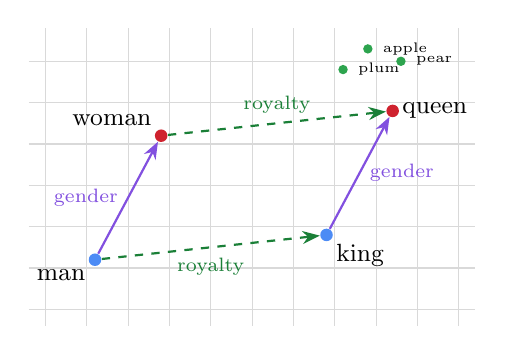
\begin{tikzpicture}[scale=1.05,
  pt/.style={circle,fill,inner sep=1.6pt},
  lbl/.style={font=\small}]
  \draw[gray!30,step=0.5] (-0.2,-0.2) grid (5.2,3.4);
  % gender direction
  \node[pt,wA] (man) at (0.6,0.6) {}; \node[lbl,below left] at (man) {man};
  \node[pt,wD] (woman) at (1.4,2.1) {}; \node[lbl,above left] at (woman) {woman};
  \node[pt,wA] (king) at (3.4,0.9) {}; \node[lbl,below right] at (king) {king};
  \node[pt,wD] (queen) at (4.2,2.4) {}; \node[lbl,right] at (queen) {queen};
  \draw[arr,wE] (man) -- node[left,font=\scriptsize]{gender} (woman);
  \draw[arr,wE] (king) -- node[right,font=\scriptsize]{gender} (queen);
  \draw[arr,okc,dashed] (man) -- node[below,font=\scriptsize]{royalty} (king);
  \draw[arr,okc,dashed] (woman) -- node[above,font=\scriptsize]{royalty} (queen);
  % a cluster
  \foreach \p/\n in {(3.9,3.15)/apple,(4.3,3.0)/pear,(3.6,2.9)/plum}
    \node[pt,wC,inner sep=1.2pt,label={[font=\tiny]right:\n}] at \p {};
\end{tikzpicture}
\end{columns}
\end{frame}

\begin{frame}{Two families before GloVe --- and the bridge}
\centering
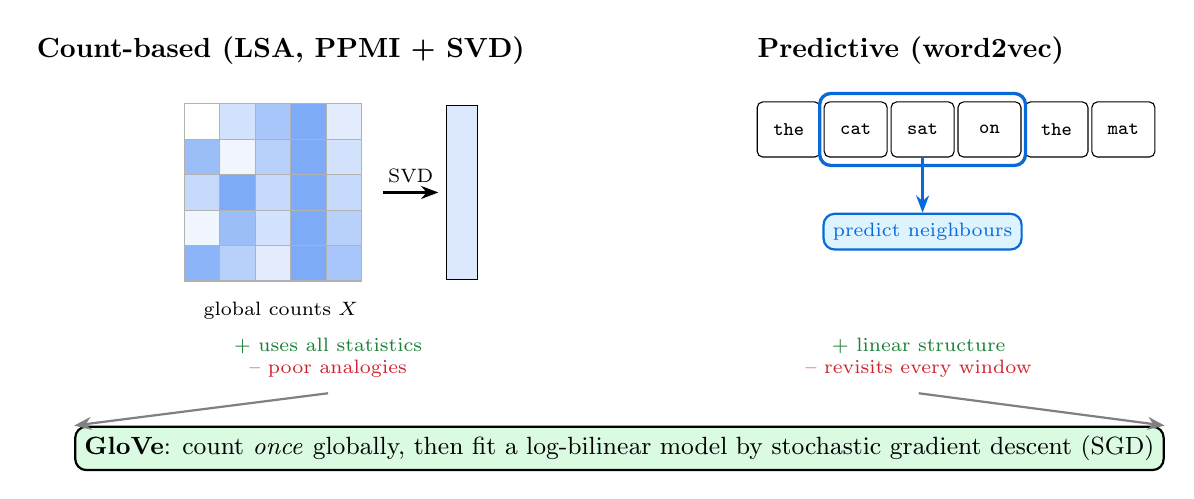
\begin{tikzpicture}[font=\small]
  % --- count based
  \node[font=\bfseries] at (0,3.3) {Count-based (LSA, PPMI + SVD)};
  \foreach \i in {0,...,4} \foreach \j in {0,...,4} {
     \pgfmathsetmacro{\v}{mod(7*\i+3*\j+\i*\j,10)*8}
     \node[cell,fill=wA!\v,minimum size=4.5mm] at (-1+\j*0.45,2.4-\i*0.45) {};}
  \node[font=\scriptsize] at (0,0.0) {global counts $X$};
  \draw[arr] (1.3,1.5) -- node[above,font=\scriptsize]{SVD} (2.0,1.5);
  \node[draw,fill=wA!20,minimum width=4mm,minimum height=22mm] at (2.3,1.5) {};
  \node[font=\scriptsize,align=center] at (0.6,-0.6) {\color{okc}+ uses all statistics\\\color{warn}-- poor analogies};
  % --- predictive
  \node[font=\bfseries] at (8,3.3) {Predictive (word2vec)};
  \foreach \w [count=\k] in {the,cat,sat,on,the,mat}
     \node[tok,minimum width=8mm,font=\scriptsize\ttfamily] (t\k) at (5.6+\k*0.85,2.3) {\w};
  \draw[very thick,accent,rounded corners] ($(t2.north west)+(-0.05,0.1)$) rectangle ($(t4.south east)+(0.05,-0.1)$);
  \draw[arr,accent] (t3.south) -- ++(0,-0.7) node[below,draw,rounded corners,fill=stageA,font=\scriptsize]{predict neighbours};
  \node[font=\scriptsize,align=center] at (8.1,-0.6) {\color{okc}+ linear structure\\\color{warn}-- revisits every window};
  % --- bridge
  \node[draw,thick,rounded corners,fill=stageD,align=center,font=\small] (g) at (4.3,-1.75)
     {\textbf{GloVe}: count \emph{once} globally, then fit a log-bilinear model by stochastic gradient descent (SGD)};
  \draw[arr,gray] (0.6,-1.05) -- (g.north west);
  \draw[arr,gray] (8.1,-1.05) -- (g.north east);
\end{tikzpicture}
\end{frame}

% =====================================================================
\section{The Model}
% =====================================================================

\begin{frame}{Meaning lives in probability \emph{ratios}}
\begin{columns}[c]
\column{0.5\textwidth}
\small
\begin{tabular}{lcc}
\toprule
probe $k$ & $\frac{P(k|\text{ice})}{P(k|\text{steam})}$ & reading\\
\midrule
solid   & \textbf{8.9}     & ice-specific\\
gas     & \textbf{0.085}   & steam-specific\\
water   & 1.36             & both\\
fashion & 0.96             & neither\\
\bottomrule
\end{tabular}

\vspace{4mm}
Raw probabilities ($10^{-5}$--$10^{-3}$) are hard to read.
The \alert{ratio} separates relevant from irrelevant probe words.

\vspace{2mm}
{\scriptsize Source: Pennington et al.\ 2014, Table 1 (6B-token corpus).}
\column{0.5\textwidth}
\centering
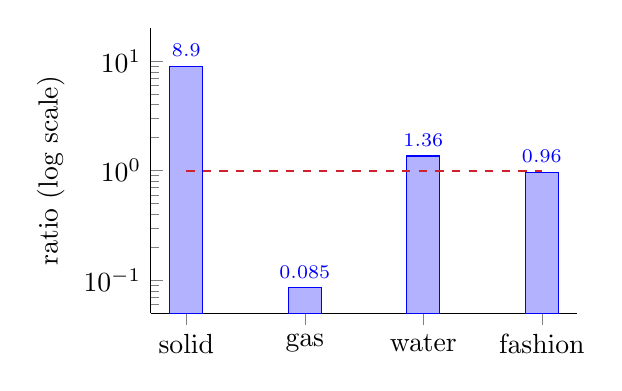
\begin{tikzpicture}
\begin{axis}[width=7cm,height=5.2cm,ybar,ymode=log,log origin=infty,
  ymin=0.05,ymax=20,bar width=12pt,
  symbolic x coords={solid,gas,water,fashion},xtick=data,
  ylabel={ratio (log scale)},axis lines*=left,
  point meta=rawy,nodes near coords,nodes near coords style={font=\scriptsize,/pgf/number format/.cd,fixed,precision=3},
  every axis plot/.append style={fill=accent!60,draw=accent}]
  \addplot coordinates {(solid,8.9) (gas,0.085) (water,1.36) (fashion,0.96)};
  \draw[dashed,warn,thick] (axis cs:solid,1) -- (axis cs:fashion,1);
\end{axis}
\end{tikzpicture}

{\scriptsize dashed line: ratio $=1$ (uninformative)}
\end{columns}
\end{frame}

\begin{frame}{From ratios to a model in three steps}
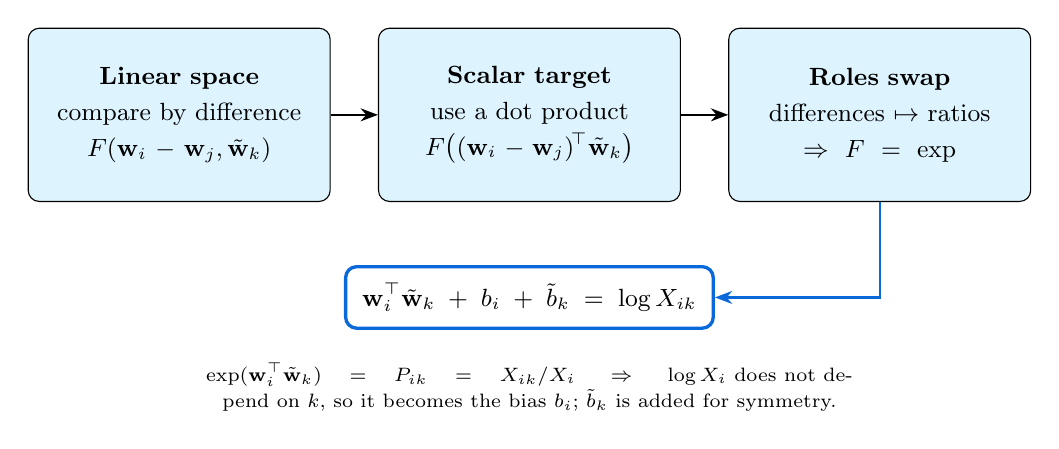
\begin{tikzpicture}[font=\small,
  st/.style={draw,rounded corners,fill=stageA,text width=36mm,minimum height=22mm,align=center}]
  \node[st] (a) at (0,0) {\textbf{Linear space}\\[2pt] compare by difference\\[2pt] $F(\wv_i-\wv_j,\cv_k)$};
  \node[st,right=6mm of a] (b) {\textbf{Scalar target}\\[2pt] use a dot product\\[2pt] $F\big((\wv_i-\wv_j)^{\!\top}\cv_k\big)$};
  \node[st,right=6mm of b] (c) {\textbf{Roles swap}\\[2pt] differences $\mapsto$ ratios\\[2pt] $\Rightarrow F=\exp$};
  \draw[arr] (a) -- (b); \draw[arr] (b) -- (c);
  \node[below=8mm of b,draw=accent,very thick,rounded corners,inner sep=6pt,fill=white] (eq)
    {$\displaystyle \wv_i^{\top}\cv_k \;+\; b_i \;+\; \tilde b_k \;=\; \log X_{ik}$};
  \draw[arr,accent] (c.south) |- (eq.east);
  \node[below=3mm of eq,font=\scriptsize,text width=120mm,align=center]
   {$\exp(\wv_i^\top\cv_k)=P_{ik}=X_{ik}/X_i$ $\;\Rightarrow\;$ $\log X_i$ does not depend on $k$, so it becomes the bias $b_i$; $\tilde b_k$ is added for symmetry.};
\end{tikzpicture}
\end{frame}

\begin{frame}{The objective: weighted least squares on $\log X$}
\begin{columns}[c]
\column{0.52\textwidth}
\[
J=\!\!\sum_{i,j:\,X_{ij}>0}\!\! f(X_{ij})\big(\underbrace{\wv_i^\top\cv_j+b_i+\tilde b_j-\log X_{ij}}_{\delta_{ij}\ \text{(\texttt{diff})}}\big)^2
\]
\[
f(x)=\begin{cases}(x/x_{\max})^{\alpha} & x<x_{\max}\\ 1 & \text{otherwise}\end{cases}
\]
\begin{itemize}\small
  \item Sum only over \alert{non-zero} cells, so the data can be stored sparse.
  \item $f(0)=0$ removes the $\log 0$ problem.
  \item Rare (noisy) pairs get small weight; frequent pairs are capped at weight 1.
  \item $\alpha=0.75$, $x_{\max}=100$ (paper); \file{demo.sh} uses $x_{\max}=10$.
\end{itemize}
\column{0.48\textwidth}
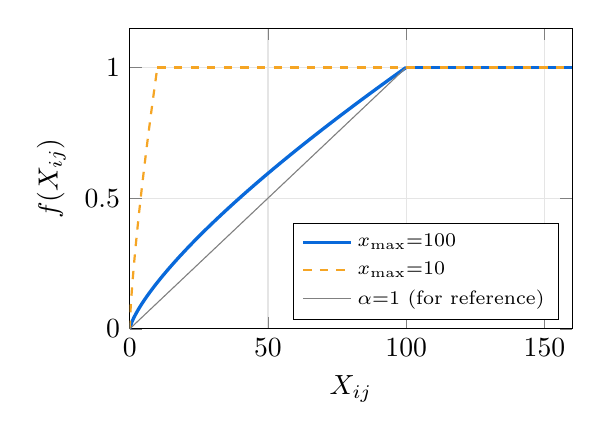
\begin{tikzpicture}
\begin{axis}[width=7.2cm,height=5.4cm,xlabel={$X_{ij}$},ylabel={$f(X_{ij})$},
  xmin=0,xmax=160,ymin=0,ymax=1.15,grid=major,grid style={gray!20},
  legend pos=south east,legend style={font=\scriptsize},legend cell align=left]
  \addplot[very thick,accent,domain=0:100,samples=150]{(x/100)^0.75};
  \addplot[very thick,accent,domain=100:160,forget plot]{1};
  \addplot[thick,dashed,wB,domain=0:10,samples=80]{(x/10)^0.75};
  \addplot[thick,dashed,wB,domain=10:160,forget plot]{1};
  \addplot[thin,gray,domain=0:100,samples=50]{x/100};
  \legend{$x_{\max}{=}100$,$x_{\max}{=}10$,$\alpha{=}1$ (for reference)}
\end{axis}
\end{tikzpicture}
\end{columns}
\end{frame}

\begin{frame}{GloVe is a weighted factorisation of $\log X$}
\centering
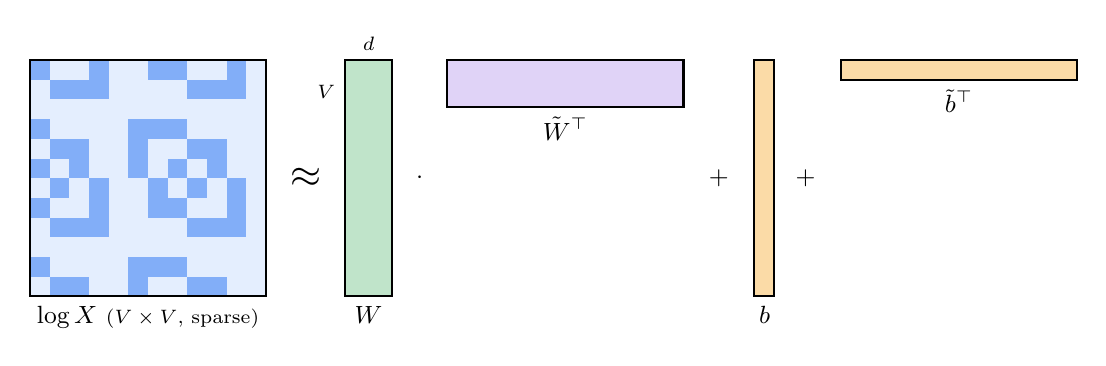
\begin{tikzpicture}[font=\small]
  % log X
  \fill[wA!15] (0,0) rectangle (3,3);
  \foreach \i in {0,...,11} \foreach \j in {0,...,11} {
     \pgfmathsetmacro{\z}{mod(\i*\j+3*\i+5*\j,7)}
     \ifdim \z pt<3pt \fill[wA!70] (\j*0.25,3-\i*0.25-0.25) rectangle ++(0.25,0.25); \fi}
  \draw[thick] (0,0) rectangle (3,3);
  \node[below] at (1.5,0) {$\log X$ \scriptsize($V\times V$, sparse)};
  \node at (3.5,1.5) {\Large$\approx$};
  % W
  \fill[wC!30] (4,0) rectangle (4.6,3); \draw[thick] (4,0) rectangle (4.6,3);
  \node[below] at (4.3,0) {$W$}; \node[left,font=\scriptsize] at (4,2.6) {$V$};
  \node[above,font=\scriptsize] at (4.3,3) {$d$};
  \node at (4.95,1.5) {$\cdot$};
  % Wt^T
  \fill[wE!25] (5.3,2.4) rectangle (8.3,3); \draw[thick] (5.3,2.4) rectangle (8.3,3);
  \node[below] at (6.8,2.4) {$\tilde W^{\top}$};
  \node at (8.75,1.5) {$+$};
  % biases
  \fill[wB!40] (9.2,0) rectangle (9.45,3); \draw[thick] (9.2,0) rectangle (9.45,3);
  \node[below] at (9.33,0) {$b$};
  \node at (9.85,1.5) {$+$};
  \fill[wB!40] (10.3,2.75) rectangle (13.3,3); \draw[thick] (10.3,2.75) rectangle (13.3,3);
  \node[below] at (11.8,2.75) {$\tilde b^{\top}$};
\end{tikzpicture}

\vspace{4mm}
\begin{itemize}\small
  \item Only the \textcolor{wA}{dark cells} (observed pairs) enter the loss, each with weight $f(X_{ij})$.
  \item Cost per epoch is $O(\mathrm{nnz}(X)\cdot d)$, where nnz is the number of non-zero cells, \alert{independent of corpus length}.
  \item There are two tables, $W$ and $\tilde W$. The default output is $\wv_i+\cv_i$, a small ensemble.
\end{itemize}
\end{frame}

\begin{frame}{Gradients (what the inner loop computes)}
\begin{columns}[c]
\column{0.5\textwidth}
With $\delta=\wv_i^\top\cv_j+b_i+\tilde b_j-\log X_{ij}$ and $g=f(X_{ij})\,\delta$ (\texttt{fdiff}):
\begin{align*}
\nabla_{\wv_i} &= g\,\cv_j & \nabla_{\cv_j} &= g\,\wv_i\\
\partial_{b_i} &= g & \partial_{\tilde b_j} &= g
\end{align*}
The reported cost is $\tfrac12 f\delta^2$, so the factor 2 drops out.
\column{0.5\textwidth}
\centering
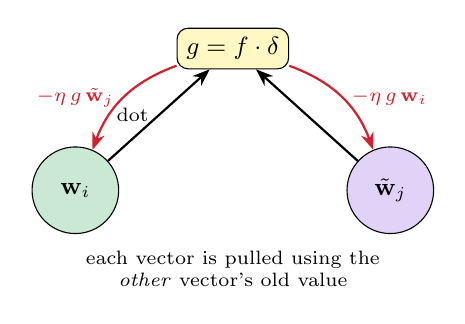
\begin{tikzpicture}[font=\small]
  \node[circle,draw,fill=wC!25,minimum size=11mm] (w) at (0,0) {$\wv_i$};
  \node[circle,draw,fill=wE!25,minimum size=11mm] (c) at (4,0) {$\cv_j$};
  \node[draw,rounded corners,fill=stageB] (d) at (2,1.8) {$g=f\cdot\delta$};
  \draw[arr] (w) -- node[left,font=\scriptsize]{dot} (d);
  \draw[arr] (c) -- (d);
  \draw[arr,warn] (d) to[bend right=25] node[left,font=\scriptsize]{$-\eta\,g\,\cv_j$} (w);
  \draw[arr,warn] (d) to[bend left=25] node[right,font=\scriptsize]{$-\eta\,g\,\wv_i$} (c);
  \node[font=\scriptsize,align=center] at (2,-1) {each vector is pulled using the\\ \emph{other} vector's old value};
\end{tikzpicture}
\end{columns}
\end{frame}

% =====================================================================
\section{The Pipeline}
% =====================================================================

\begin{frame}{Four Unix filters, connected by files}
\centering
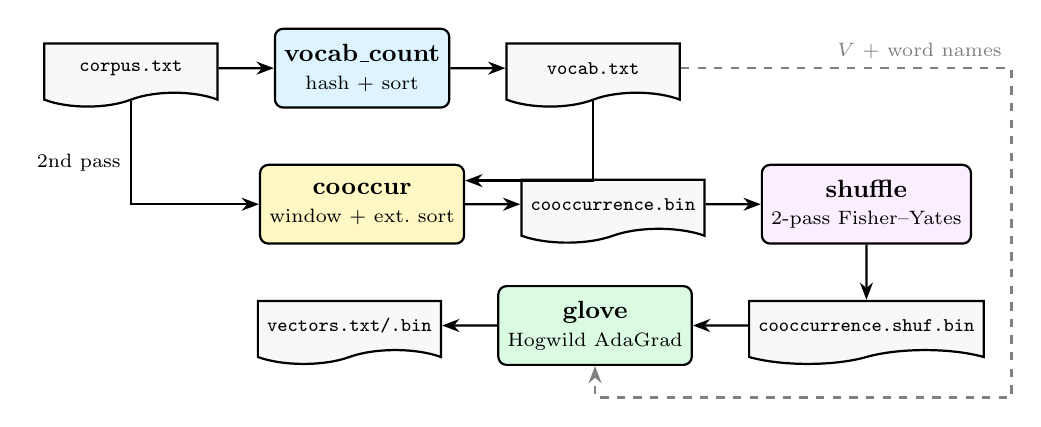
\begin{tikzpicture}[node distance=5mm and 7mm]
  \node[data] (corpus) {corpus.txt};
  \node[tool,fill=stageA,right=of corpus] (vc) {\textbf{vocab\_count}\\[-1pt]{\scriptsize hash + sort}};
  \node[data,right=of vc] (vocab) {vocab.txt};
  \node[tool,fill=stageB,below=7mm of vc] (co) {\textbf{cooccur}\\[-1pt]{\scriptsize window + ext.\ sort}};
  \node[data,right=of co] (cbin) {cooccurrence.bin};
  \node[tool,fill=stageC,right=of cbin] (sh) {\textbf{shuffle}\\[-1pt]{\scriptsize 2-pass Fisher--Yates}};
  \node[data,below=7mm of sh] (sbin) {cooccurrence.shuf.bin};
  \node[tool,fill=stageD,left=of sbin] (gl) {\textbf{glove}\\[-1pt]{\scriptsize Hogwild AdaGrad}};
  \node[data,left=of gl] (vec) {vectors.txt/.bin};
  \draw[arr] (corpus) -- (vc);
  \draw[arr] (vc) -- (vocab);
  \draw[arr] (corpus) |- node[pos=0.3,left,font=\scriptsize]{2nd pass} (co);
  \draw[arr] (vocab) |- ($(co.east)+(0,3mm)$);
  \draw[arr] (co) -- (cbin);
  \draw[arr] (cbin) -- (sh);
  \draw[arr] (sh) -- (sbin);
  \draw[arr] (sbin) -- (gl);
  \draw[arr] (gl) -- (vec);
  \coordinate (X) at ($(sh.east)+(5mm,0)$);
  \draw[arr,dashed,gray] (vocab.east) -- (vocab.east -| X) |- ($(gl.south)+(0,-4mm)$) -- (gl.south);
  \node[font=\scriptsize,gray,anchor=south east] at (vocab.east -| X) {$V$ + word names};
\end{tikzpicture}

\vspace{3mm}
\small
\begin{itemize}
  \item Each tool reads standard input (\texttt{stdin}) or files, writes standard output (\texttt{stdout}), and logs to standard error (\texttt{stderr}). There is no shared state.
  \item Any stage can be re-run alone (e.g.\ retrain with a new $d$ without recounting).
  \item Every stage except \texttt{glove} works \alert{out of core}.
\end{itemize}
\end{frame}

\begin{frame}[fragile]{Running it end to end (\file{demo.sh})}
\begin{lstlisting}[style=sh]
make                                          # -> build/{vocab_count,cooccur,shuffle,glove}
build/vocab_count -min-count 5 -verbose 2                    < text8 > vocab.txt
build/cooccur -memory 4.0 -vocab-file vocab.txt -window-size 15 < text8 > cooccurrence.bin
build/shuffle -memory 4.0                        < cooccurrence.bin > cooccurrence.shuf.bin
build/glove -save-file vectors -threads 8 -input-file cooccurrence.shuf.bin \
            -x-max 10 -iter 15 -vector-size 50 -binary 2 -vocab-file vocab.txt
python eval/python/evaluate.py                # analogy accuracy
\end{lstlisting}
\begin{columns}[T]
\column{0.5\textwidth}\small
\begin{itemize}
  \item text8 is about 17M tokens; the demo runs in minutes.
  \item The 2024 Wiki+Gigaword runs used \opt{min-count}~20, \opt{window-size}~10, and 50--100 iterations.
\end{itemize}
\column{0.5\textwidth}\small
\begin{itemize}
  \item The corpus must be \alert{pre-tokenised} and whitespace-separated.
  \item A newline marks a \alert{document boundary}: context windows never cross it.
\end{itemize}
\end{columns}
\end{frame}

\begin{frame}{The universal record: \texttt{CREC} (co-occurrence record, 16 bytes)}
\centering
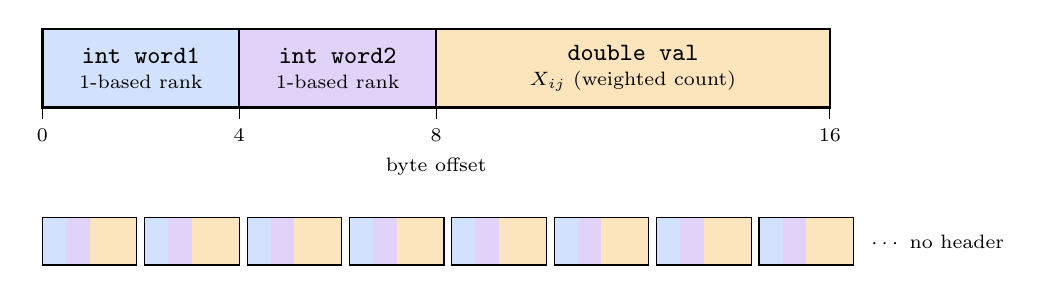
\begin{tikzpicture}[font=\small]
  \draw[thick,fill=wA!25] (0,0) rectangle (2.5,1) node[midway,align=center]{\texttt{int word1}\\[-2pt]\scriptsize 1-based rank};
  \draw[thick,fill=wE!25] (2.5,0) rectangle (5,1) node[midway,align=center]{\texttt{int word2}\\[-2pt]\scriptsize 1-based rank};
  \draw[thick,fill=wB!30] (5,0) rectangle (10,1) node[midway,align=center]{\texttt{double val}\\[-2pt]\scriptsize $X_{ij}$ (weighted count)};
  \foreach \x/\b in {0/0,2.5/4,5/8,10/16} {\draw (\x,0) -- (\x,-0.15); \node[below,font=\scriptsize] at (\x,-0.15) {\b};}
  \node[font=\scriptsize] at (5,-0.75) {byte offset};
  % stream
  \foreach \k in {0,...,7} {
    \draw[fill=white] (\k*1.3,-2) rectangle ++(1.2,0.6);
    \fill[wA!25] (\k*1.3,-2) rectangle ++(0.3,0.6);
    \fill[wE!25] (\k*1.3+0.3,-2) rectangle ++(0.3,0.6);
    \fill[wB!30] (\k*1.3+0.6,-2) rectangle ++(0.6,0.6);
    \draw (\k*1.3,-2) rectangle ++(1.2,0.6);}
  \node[right,font=\scriptsize] at (10.4,-1.7) {$\cdots$ no header};
\end{tikzpicture}

\vspace{4mm}
\begin{itemize}\small
  \item Files written by \texttt{cooccur} and \texttt{shuffle} and read by \texttt{glove} are raw \texttt{fwrite}s of \texttt{CREC} arrays.
  \item $\text{size}=16\cdot\mathrm{nnz}(X)$. \texttt{glove} computes the record count as \texttt{filesize/16}.
  \item The layout is native-endian and \alert{not portable} across architectures.
\end{itemize}
\end{frame}

% =====================================================================
\section{Stage 1: vocab\_count}
% =====================================================================

\begin{frame}{Counting words: hash table with move-to-front}
\begin{columns}[c]
\column{0.55\textwidth}
\centering
\begin{tikzpicture}[font=\scriptsize,
  b/.style={draw,minimum width=8mm,minimum height=5mm,fill=gray!10},
  r/.style={draw,rounded corners=1pt,minimum width=13mm,minimum height=5mm,fill=white}]
  \foreach \i in {0,...,5} \node[b] (b\i) at (0,-\i*0.6) {\i};
  \node[above,font=\scriptsize] at (b0.north) {$2^{20}$ buckets};
  \only<1>{
  \node[r,right=5mm of b2] (x1) {the:912};
  \node[r,right=3mm of x1] (x2) {of:540};
  \node[r,right=3mm of x2,fill=wB!40] (x3) {sat:17};
  \draw[arr] (b2) -- (x1); \draw[arr] (x1) -- (x2); \draw[arr] (x2) -- (x3);
  \node[below=2mm of x3,font=\scriptsize,warn] {lookup ``sat'': 3 steps};}
  \only<2>{
  \node[r,right=5mm of b2,fill=wB!40] (x3) {sat:18};
  \node[r,right=3mm of x3] (x1) {the:912};
  \node[r,right=3mm of x1] (x2) {of:540};
  \draw[arr] (b2) -- (x3); \draw[arr] (x3) -- (x1); \draw[arr] (x1) -- (x2);
  \node[below=2mm of x2,font=\scriptsize,okc] {moved to front};}
  \node[r,right=5mm of b0] (y1) {cat:40}; \draw[arr] (b0) -- (y1);
  \node[r,right=5mm of b4] (z1) {mat:9}; \draw[arr] (b4) -- (z1);
\end{tikzpicture}
\column{0.45\textwidth}\small
\begin{itemize}
  \item \texttt{bitwisehash}: shift-xor string hash.
  \item Separate chaining. A hit is \alert{moved to the front} of its chain.
  \item Under Zipf's law a few words get most lookups, so they stay at the front and lookups are close to $O(1)$.
  \item Then the words are sorted by count desc (ties alphabetical) and the list is truncated by \opt{min-count}/\opt{max-vocab}.
\end{itemize}
\end{columns}
\end{frame}

\begin{frame}{The \file{vocab.txt} contract: \emph{line number = word id}}
\centering
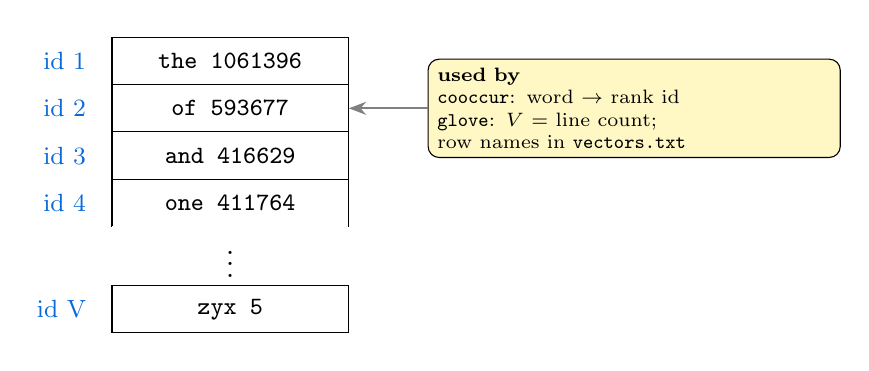
\begin{tikzpicture}[font=\small\ttfamily]
  \matrix (m) [matrix of nodes,nodes={draw,minimum width=30mm,minimum height=6mm,anchor=west,fill=white},
     column sep=0pt,row sep=-\pgflinewidth] {
     the 1061396\\ of 593677\\ and 416629\\ one 411764\\ |[fill=white,draw=none]| \vdots\\ zyx 5\\};
  \foreach \r/\id in {1/1,2/2,3/3,4/4,6/V}
     \node[left=2mm of m-\r-1,font=\small\rmfamily,accent] {id \id};
  \node[right=10mm of m-2-1,draw,rounded corners,fill=stageB,font=\scriptsize\rmfamily,align=left,text width=50mm] (u)
    {\textbf{used by}\\ \texttt{cooccur}: word $\to$ rank id\\ \texttt{glove}: $V$ = line count;\\ row names in \file{vectors.txt}};
  \draw[arr,gray] (u.west) -- (m-2-1.east);
\end{tikzpicture}

\vspace{3mm}
\small
\begin{itemize}
  \item Id 1 is the most frequent word. Small ids are the hot words, which \texttt{cooccur} exploits.
  \item The literal token \texttt{<unk>} is \alert{forbidden} in the corpus because it is reserved for the output.
  \item Never edit \file{vocab.txt} between stages.
\end{itemize}
\end{frame}

% =====================================================================
\section{Stage 2: cooccur}
% =====================================================================

\begin{frame}{Sliding the window (symmetric, $W{=}2$, weight $1/\text{distance}$)}
\centering
\begin{tikzpicture}
  \only<1>{\winstep{1}{0/1}{target \texttt{cat}: $X_{\text{the,cat}}\mathrel{+}=1$ \ (and the transpose)}}
  \only<2>{\winstep{2}{1/1,0/$\frac12$}{target \texttt{sat}: $X_{\text{cat,sat}}\mathrel{+}=1,\ X_{\text{the,sat}}\mathrel{+}=\frac12$}}
  \only<3>{\winstep{3}{2/1,1/$\frac12$}{target \texttt{on}: $X_{\text{sat,on}}\mathrel{+}=1,\ X_{\text{cat,on}}\mathrel{+}=\frac12$}}
  \only<4>{\winstep{4}{3/1,2/$\frac12$}{target \texttt{the}: $X_{\text{on,the}}\mathrel{+}=1,\ X_{\text{sat,the}}\mathrel{+}=\frac12$}}
  \only<5>{\winstep{5}{4/1,3/$\frac12$}{target \texttt{mat}: $X_{\text{the,mat}}\mathrel{+}=1,\ X_{\text{on,mat}}\mathrel{+}=\frac12$}}
  \draw[white] (-0.6,1.6) rectangle (9.5,-1.5);
\end{tikzpicture}

\vspace{2mm}
\small
\begin{itemize}
  \item The tool only looks \alert{left}, using a circular \texttt{history[W]} buffer. ``Symmetric'' adds $X_{ji}$ as well.
  \item Out-of-vocabulary tokens are skipped completely: they do not take a slot or count toward distance.
  \item A newline resets the window.
\end{itemize}
\end{frame}

\begin{frame}{Result: the co-occurrence matrix of the example}
\begin{columns}[c]
\column{0.5\textwidth}
\centering
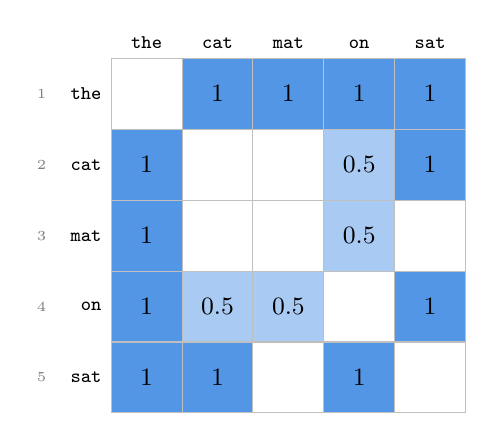
\begin{tikzpicture}
  \def\names{the,cat,mat,on,sat}
  \def\M{{0,1,1,1,1},{1,0,0,0.5,1},{1,0,0,0.5,0},{1,0.5,0.5,0,1},{1,1,0,1,0}}
  \foreach \r [count=\i from 0] in {{0,1,1,1,1},{1,0,0,0.5,1},{1,0,0,0.5,0},{1,0.5,0.5,0,1},{1,1,0,1,0}} {
    \foreach \v [count=\j from 0] in \r {
      \pgfmathsetmacro{\pc}{\v*70}
      \node[draw=gray!50,minimum size=9mm,fill=accent!\pc,font=\small] at (\j*0.9,-\i*0.9)
         {\ifdim\v pt>0pt $\v$\fi};
    }}
  \foreach \n [count=\j from 0] in \names {
    \node[font=\scriptsize\ttfamily,above] at (\j*0.9,0.45) {\n};
    \node[font=\scriptsize\ttfamily,left] at (-0.45,-\j*0.9) {\n};
    \node[font=\tiny,gray,left] at (-1.15,-\j*0.9) {\pgfmathparse{int(\j+1)}\pgfmathresult};}
\end{tikzpicture}
\column{0.5\textwidth}\small
\begin{itemize}
  \item Ids: the=1, then ties alphabetical: cat=2, mat=3, on=4, sat=5.
  \item The matrix is symmetric because the context is symmetric.
  \item $X_{\text{the,sat}}=\frac12+\frac12$ comes from two distance-2 hits.
  \item 16 non-zero cells, so 16 \texttt{CREC}s $=$ 256 bytes.
  \item The diagonal and empty cells are \alert{never stored}.
\end{itemize}
\end{columns}
\end{frame}

\begin{frame}{Zipf $\Rightarrow$ split the matrix by rank product}
\begin{columns}[c]
\column{0.5\textwidth}
\centering
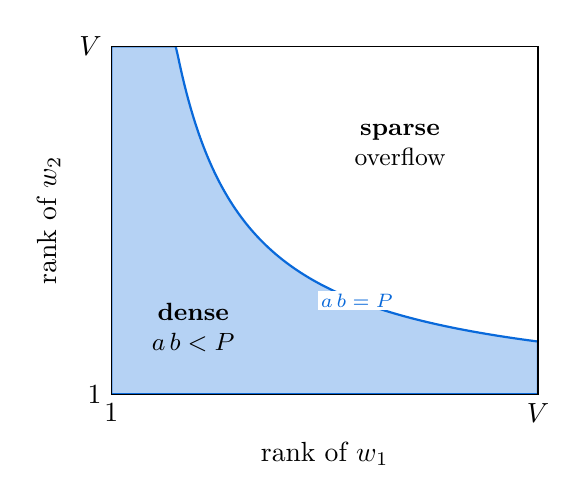
\begin{tikzpicture}
\begin{axis}[width=7cm,height=6cm,xmin=1,xmax=100,ymin=1,ymax=100,
  xlabel={rank of $w_1$},ylabel={rank of $w_2$},axis on top,
  xtick={1,100},xticklabels={1,$V$},ytick={1,100},yticklabels={1,$V$}]
  \addplot[fill=accent!30,draw=accent,thick,domain=1:100,samples=200]{min(100,1600/x)} \closedcycle;
  \node[font=\small,align=center] at (axis cs:20,20) {\textbf{dense}\\$a\,b<P$};
  \node[font=\small,align=center] at (axis cs:68,72) {\textbf{sparse}\\overflow};
  \node[font=\scriptsize,accent,fill=white,inner sep=1pt] at (axis cs:58,27.6) {$a\,b=P$};
\end{axis}
\end{tikzpicture}
\column{0.5\textwidth}\small
\begin{itemize}
  \item Count of the rank-$r$ word $\propto 1/r$, so $\mathbb E[X_{ab}]$ falls roughly like $1/(ab)$.
  \item \textbf{Dense region} (small $ab$): hot and heavily filled. Stored in a ragged array and updated \alert{in place}.
  \item \textbf{Sparse region}: cold, long tail. Appended to a buffer, then sorted and spilled to disk.
  \item $P=$ \texttt{max\_product}, derived from \opt{memory}.
\end{itemize}
\end{columns}
\end{frame}

\begin{frame}[fragile]{The dense part: a ragged array + prefix sums}
\begin{columns}[c]
\column{0.55\textwidth}
\centering
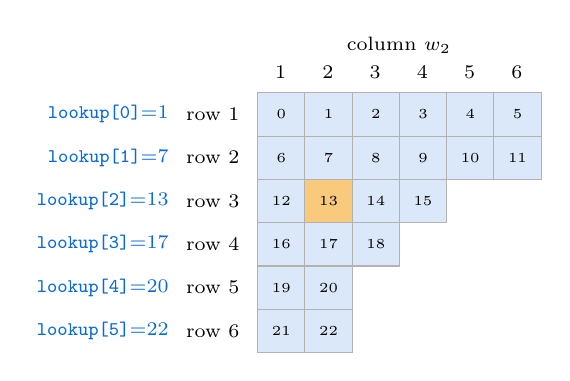
\begin{tikzpicture}[font=\tiny]
  % P=12, V=6 -> row lengths 6,6,4,3,2,2 ; lookup 1,7,13,17,20,22,24
  \def\off{0}
  \foreach \a/\len/\lk/\st in {1/6/1/0,2/6/7/6,3/4/13/12,4/3/17/16,5/2/20/19,6/2/22/21} {
    \node[font=\scriptsize,anchor=east] at (-0.1,-\a*0.55+0.27) {row \a};
    \node[font=\scriptsize,accent,anchor=east] at (-1.0,-\a*0.55+0.27) {\texttt{lookup[\the\numexpr\a-1\relax]}=\lk};
    \foreach \b in {1,...,\len} {
      \pgfmathtruncatemacro{\o}{\st+\b-1}
      \ifnum\a=3 \ifnum\b=2
        \node[cell,minimum width=6mm,minimum height=5.5mm,fill=wB!60,anchor=north west] at (\b*0.6-0.6,-\a*0.55+0.55) {\o};
      \else
        \node[cell,minimum width=6mm,minimum height=5.5mm,fill=accent!15,anchor=north west] at (\b*0.6-0.6,-\a*0.55+0.55) {\o};
      \fi\else
        \node[cell,minimum width=6mm,minimum height=5.5mm,fill=accent!15,anchor=north west] at (\b*0.6-0.6,-\a*0.55+0.55) {\o};
      \fi}
  }
  \foreach \b in {1,...,6} \node[font=\scriptsize] at (\b*0.6-0.3,0.25) {\b};
  \node[font=\scriptsize] at (1.8,0.6) {column $w_2$};
\end{tikzpicture}

{\scriptsize Toy example: $P=12$, $V=6$; cells show the offset in \texttt{bigram\_table}.}
\column{0.45\textwidth}
\begin{lstlisting}[style=c]
lookup[0] = 1;
for (a = 1; a <= V; a++)
  lookup[a] = lookup[a-1]
            + min(P / a, V);
// cell (w1,w2), 1-based:
bigram_table[lookup[w1-1]
             + w2 - 2] += 1.0/dist;
\end{lstlisting}
\small
Highlighted: $(3,2)\mapsto 13+2-2=13$.\\
Row $a$ holds $\min(\lfloor P/a\rfloor,V)$ cells.
\end{columns}
\end{frame}

\begin{frame}{The sparse part: spill sorted runs, then a $k$-way merge}
\centering
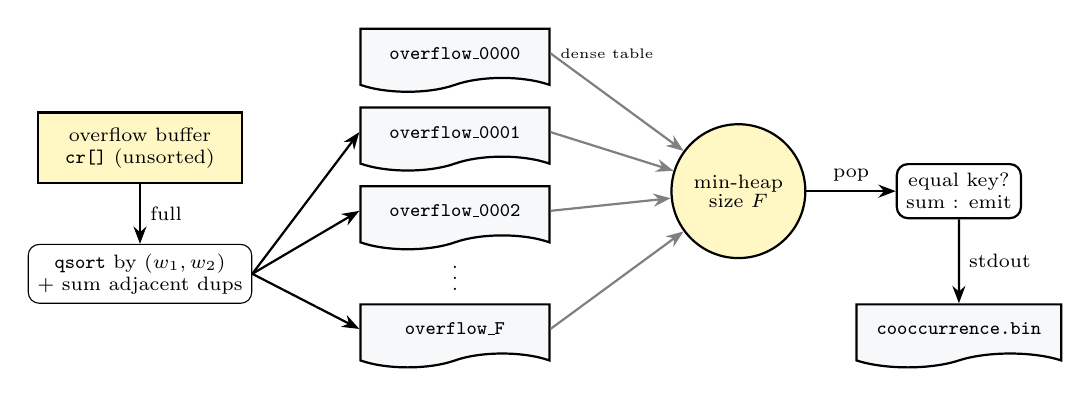
\begin{tikzpicture}[font=\scriptsize]
  % buffer
  \node[draw,thick,fill=stageB,minimum width=26mm,minimum height=9mm,align=center] (buf) at (0,0) {overflow buffer\\\texttt{cr[]} (unsorted)};
  \node[draw,rounded corners,fill=white,align=center] (srt) at (0,-1.6) {\texttt{qsort} by $(w_1,w_2)$\\+ sum adjacent dups};
  \draw[arr] (buf) -- node[right]{full} (srt);
  % files
  \node[data,minimum width=24mm] (f0) at (4,1.2) {overflow\_0000};
  \node[font=\tiny,right] at (f0.east) {dense table};
  \node[data,minimum width=24mm] (f1) at (4,0.2) {overflow\_0001};
  \node[data,minimum width=24mm] (f2) at (4,-0.8) {overflow\_0002};
  \node at (4,-1.55) {$\vdots$};
  \node[data,minimum width=24mm] (fn) at (4,-2.3) {overflow\_F};
  \draw[arr] (srt.east) -- (f1.west); \draw[arr] (srt.east) -- (f2.west); \draw[arr] (srt.east) -- (fn.west);
  % heap
  \node[draw,circle,thick,fill=stageB,minimum size=17mm,align=center] (h) at (7.6,-0.55) {min-heap\\[-1pt]size $F$};
  \foreach \n in {f0,f1,f2,fn} \draw[arr,gray] (\n.east) -- (h);
  \node[draw,rounded corners,thick,align=center] (acc) at (10.4,-0.55) {equal key?\\sum : emit};
  \draw[arr] (h) -- node[above]{pop} (acc);
  \node[data,minimum width=26mm] (out) at (10.4,-2.3) {cooccurrence.bin};
  \draw[arr] (acc) -- node[right]{stdout} (out);
\end{tikzpicture}

\vspace{3mm}
\small The output is \alert{globally sorted with unique $(w_1,w_2)$ keys}, and temp files are deleted afterwards.
More \opt{memory} means more pairs take the dense path and fewer files are merged. The \emph{output is identical} either way.
\end{frame}

\begin{frame}{Turning \opt{memory} into buffer sizes}
\begin{columns}[c]
\column{0.55\textwidth}
\[
R=\frac{0.85\cdot M\cdot 2^{30}}{16},\qquad \texttt{overflow\_length}=R/6
\]
Solve for $P$ by fixed-point iteration:
\[
P\,(\ln P + \underbrace{0.1544313298}_{2\gamma-1}) = R
\]
\small
Number of integer pairs with $ab\le P$ $=\sum_{k\le P}d(k)\approx P\ln P+(2\gamma-1)P$ (Dirichlet divisor estimate).
This sizes the hyperbolic dense region.
\column{0.45\textwidth}
\centering
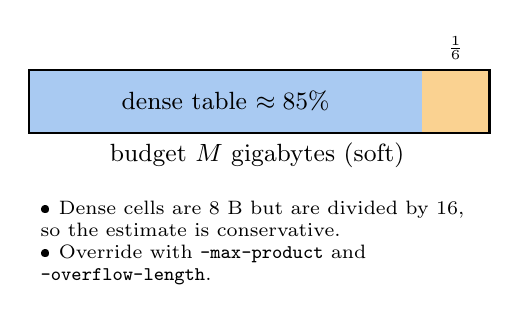
\begin{tikzpicture}
  \fill[accent!35] (0,0) rectangle (5,0.8);
  \node[font=\small] at (2.5,0.4) {dense table $\approx 85\%$};
  \fill[wB!50] (5,0) rectangle (5.85,0.8);
  \node[font=\scriptsize,above] at (5.42,0.8) {$\tfrac16$};
  \draw[thick] (0,0) rectangle (5.85,0.8);
  \node[font=\small,below] at (2.9,0) {budget $M$ gigabytes (soft)};
  \node[font=\scriptsize,align=left,text width=55mm] at (2.9,-1.4)
   {\textbullet\ Dense cells are 8 B but are divided by 16, so the estimate is conservative.\\
    \textbullet\ Override with \opt{max-product} and \opt{overflow-length}.};
\end{tikzpicture}
\end{columns}
\end{frame}

% =====================================================================
\section{Stage 3: shuffle}
% =====================================================================

\begin{frame}{Why shuffle? Sorted input breaks SGD}
\centering
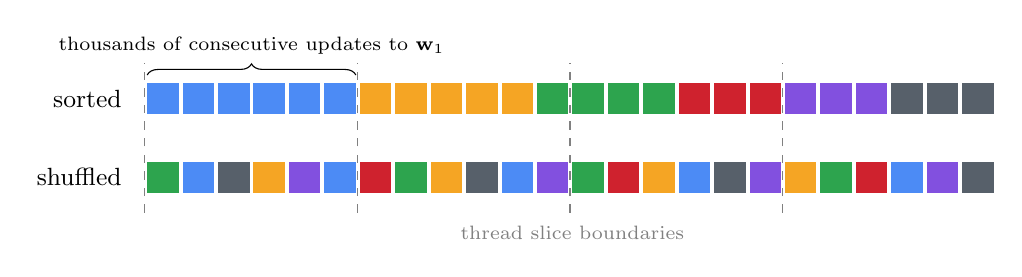
\begin{tikzpicture}
  \def\sorted{A,A,A,A,A,A,B,B,B,B,B,C,C,C,C,D,D,D,E,E,E,F,F,F}
  \def\shuf{C,A,F,B,E,A,D,C,B,F,A,E,C,D,B,A,F,E,B,C,D,A,E,F}
  \node[font=\small,anchor=east] at (-0.2,0) {sorted};
  \foreach \c [count=\i from 0] in \sorted \fill[w\c] (\i*0.45,-0.2) rectangle ++(0.4,0.4);
  \node[font=\small,anchor=east] at (-0.2,-1) {shuffled};
  \foreach \c [count=\i from 0] in \shuf \fill[w\c] (\i*0.45,-1.2) rectangle ++(0.4,0.4);
  \draw[decorate,decoration={brace,amplitude=4pt}] (0,0.3) -- node[above=4pt,font=\scriptsize]{thousands of consecutive updates to $\wv_1$} (2.65,0.3);
  % thread slices
  \foreach \t in {0,1,2,3} \draw[dashed,gray] (\t*2.7-0.03,-1.45) -- (\t*2.7-0.03,0.45);
  \node[font=\scriptsize,gray] at (5.4,-1.7) {thread slice boundaries};
\end{tikzpicture}

\vspace{3mm}
\small
\begin{itemize}
  \item \texttt{cooccurrence.bin} is sorted by $w_1$, i.e.\ grouped by word (one colour per word).
  \item In sorted order, the updates are \alert{biased}: one row is hammered, then the next.
  \item Sorted order also causes \alert{contention} between Hogwild threads. After shuffling, consecutive and concurrent updates touch different rows.
\end{itemize}
\end{frame}

\begin{frame}{Out-of-core shuffle in two passes}
\centering
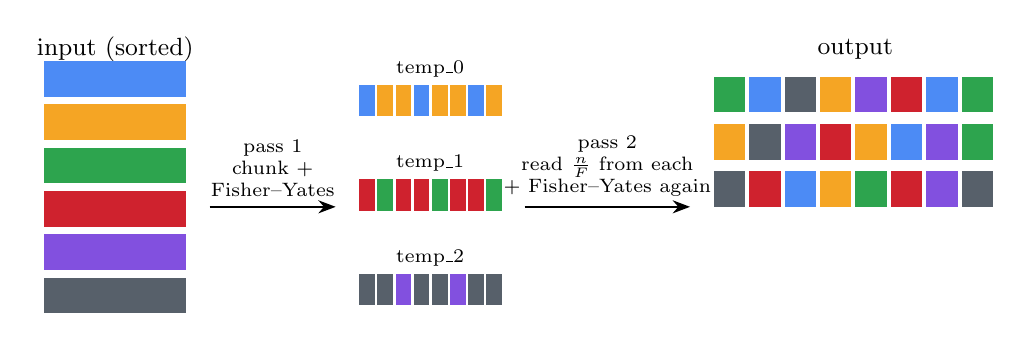
\begin{tikzpicture}[font=\scriptsize]
  \def\cols{A,B,C,D,E,F}
  % input
  \node[font=\small] at (0.9,2.4) {input (sorted)};
  \foreach \c [count=\i from 0] in \cols \fill[w\c] (0,1.8-\i*0.55) rectangle ++(1.8,0.45);
  % pass 1
  \draw[arr] (2.1,0.4) -- node[above,align=center]{pass 1\\chunk +\\Fisher--Yates} (3.7,0.4);
  \foreach \k/\a/\b in {0/A/B,1/C/D,2/E/F} {
    \node[font=\scriptsize] at (4.9,2.15-\k*1.2) {temp\_\k};
    \foreach \j in {0,...,7} {
      \pgfmathtruncatemacro{\pick}{mod(\j*5+\k,3)}
      \ifnum\pick=0 \fill[w\a] (4+\j*0.23,1.55-\k*1.2) rectangle ++(0.2,0.4);
      \else \fill[w\b] (4+\j*0.23,1.55-\k*1.2) rectangle ++(0.2,0.4); \fi}}
  % pass 2
  \draw[arr] (6.1,0.4) -- node[above,align=center]{pass 2\\read $\frac{n}{F}$ from each\\+ Fisher--Yates again} (8.2,0.4);
  \node[font=\small] at (10.3,2.4) {output};
  \def\mix{C,A,F,B,E,D,A,C,B,F,E,D,B,A,E,C,F,D,A,B,C,D,E,F}
  \foreach \c [count=\i from 0] in \mix {
     \pgfmathtruncatemacro{\r}{int(\i/8)} \pgfmathtruncatemacro{\cc}{mod(\i,8)}
     \fill[w\c] (8.5+\cc*0.45,1.6-\r*0.6) rectangle ++(0.4,0.45);}
\end{tikzpicture}

\vspace{3mm}
\small
\begin{itemize}
  \item Chunk size $=0.95\,M\cdot 2^{30}/16$ records. Fisher--Yates with \texttt{rand\_long} (rejection sampling, so no modulo bias).
  \item The result is not a perfectly uniform permutation (``good enough''), but every output window mixes the whole input.
  \item \opt{seed} makes it reproducible; the default seed is \texttt{time(0)}.
\end{itemize}
\end{frame}

% =====================================================================
\section{Stage 4: glove, the trainer}
% =====================================================================

\begin{frame}{All parameters in one aligned array}
\centering
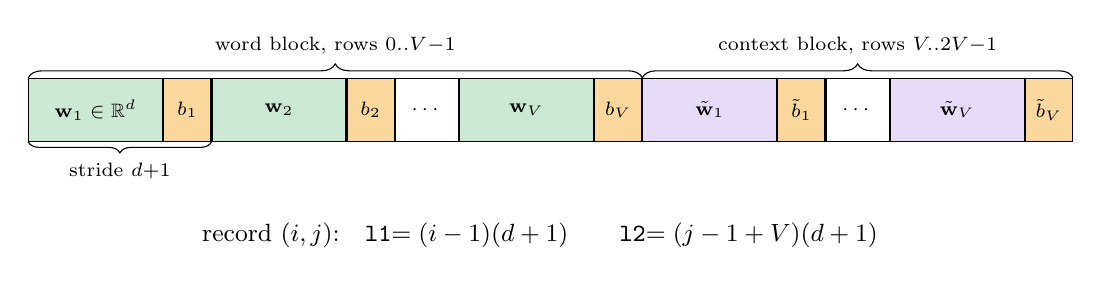
\begin{tikzpicture}[font=\scriptsize,
  c/.style={draw,minimum height=8mm,inner sep=1pt,anchor=west},
  v/.style={c,fill=wC!25,minimum width=17mm},
  b/.style={c,fill=wB!45,minimum width=6mm},
  cv/.style={c,fill=wE!20,minimum width=17mm}]
  \node[v] (w1) at (0,0) {$\wv_1\in\mathbb R^d$};
  \node[b] (b1) at (w1.east) {$b_1$};
  \node[v] (w2) at (b1.east) {$\wv_2$};
  \node[b] (b2) at (w2.east) {$b_2$};
  \node[c,minimum width=8mm] (d1) at (b2.east) {$\cdots$};
  \node[v] (wV) at (d1.east) {$\wv_V$};
  \node[b] (bV) at (wV.east) {$b_V$};
  \node[cv] (c1) at (bV.east) {$\cv_1$};
  \node[b] (cb1) at (c1.east) {$\tilde b_1$};
  \node[c,minimum width=8mm] (d2) at (cb1.east) {$\cdots$};
  \node[cv] (cV) at (d2.east) {$\cv_V$};
  \node[b] (cbV) at (cV.east) {$\tilde b_V$};
  \draw[decorate,decoration={brace,amplitude=5pt}] (w1.north west) -- node[above=5pt]{word block, rows $0..V{-}1$} (bV.north east);
  \draw[decorate,decoration={brace,amplitude=5pt}] (c1.north west) -- node[above=5pt]{context block, rows $V..2V{-}1$} (cbV.north east);
  \draw[decorate,decoration={brace,mirror,amplitude=4pt}] (w1.south west) -- node[below=4pt]{stride $d{+}1$} (b1.south east);
  \node[font=\small,align=center] at (6.5,-1.6) {record $(i,j)$:\quad
     \texttt{l1}$=(i-1)(d+1)$\qquad \texttt{l2}$=(j-1+V)(d+1)$};
\end{tikzpicture}

\vspace{3mm}
\small
\begin{itemize}
  \item \texttt{W} and \texttt{gradsq} each hold $2V(d+1)$ doubles, aligned with \texttt{posix\_memalign(128)}.
  \item The bias sits next to its vector, so they share cache lines.
  \item Initialisation: $W\sim\mathcal U(-0.5,0.5)/d$, $\texttt{gradsq}=1$, or loaded from a checkpoint.
\end{itemize}
\end{frame}

\begin{frame}{One SGD step, as a pipeline}
\centering
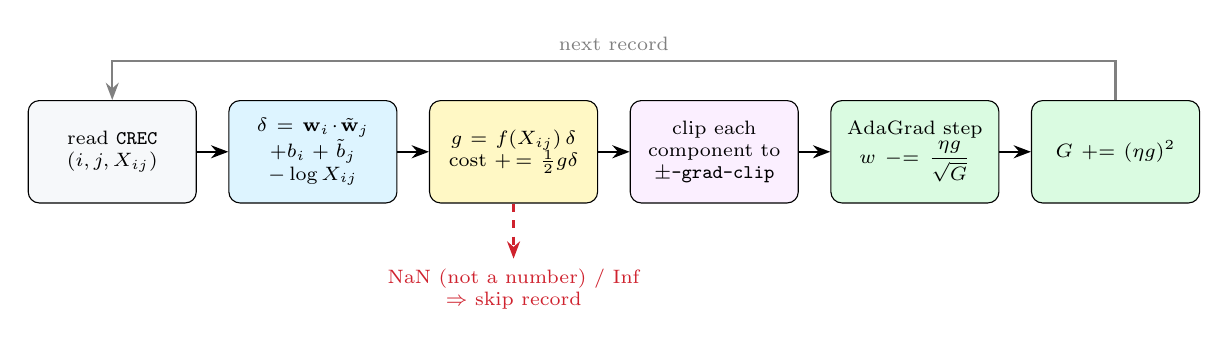
\begin{tikzpicture}[font=\scriptsize,node distance=4mm,
  s/.style={draw,rounded corners,fill=stageA,align=center,minimum height=13mm,text width=19mm}]
  \node[s,fill=fileC] (r) {read \texttt{CREC}\\$(i,j,X_{ij})$};
  \node[s,right=of r] (d) {$\delta=\wv_i\!\cdot\!\cv_j$\\$+b_i+\tilde b_j$\\$-\log X_{ij}$};
  \node[s,right=of d,fill=stageB] (f) {$g=f(X_{ij})\,\delta$\\cost $+\!=\tfrac12 g\delta$};
  \node[s,right=of f,fill=stageC] (c) {clip each\\component to\\$\pm$\opt{grad-clip}};
  \node[s,right=of c,fill=stageD] (a) {AdaGrad step\\$w\mathrel{-}=\dfrac{\eta g}{\sqrt{G}}$};
  \node[s,right=of a,fill=stageD] (u) {$G\mathrel{+}=(\eta g)^2$};
  \draw[arr] (r) -- (d); \draw[arr] (d) -- (f); \draw[arr] (f) -- (c); \draw[arr] (c) -- (a); \draw[arr] (a) -- (u);
  \draw[arr,warn,dashed] (f.south) -- ++(0,-0.7) node[below,align=center,warn]{NaN (not a number) / Inf\\$\Rightarrow$ skip record};
  \draw[arr,gray] (u.north) -- ++(0,0.5) -| node[pos=0.25,above,gray]{next record} (r.north);
\end{tikzpicture}

\vspace{5mm}
\small
\begin{columns}[T]
\column{0.5\textwidth}
\begin{itemize}
  \item Both vector updates are computed from \emph{old} values, then applied together.
  \item $G$ starts at 1, so the first step size is exactly $\eta\,g$.
\end{itemize}
\column{0.5\textwidth}
\begin{itemize}
  \item \alert{Biases}: $b\mathrel{-}=g/\sqrt G$, with no $\eta$ and no clipping.
  \item The divisor uses $G$ \emph{before} this step's gradient is added.
\end{itemize}
\end{columns}
\end{frame}

\begin{frame}{AdaGrad: frequent words slow down, rare words keep learning}
\begin{columns}[c]
\column{0.55\textwidth}
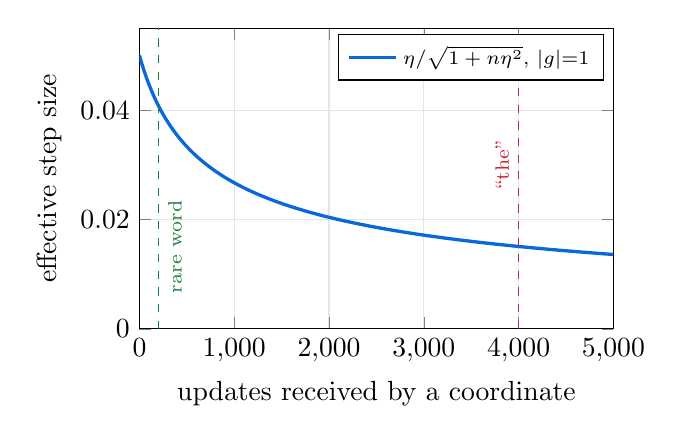
\begin{tikzpicture}
\begin{axis}[width=7.6cm,height=5.4cm,xlabel={updates received by a coordinate},
  ylabel={effective step size},xmin=0,xmax=5000,ymin=0,ymax=0.055,
  scaled y ticks=false,yticklabel style={/pgf/number format/fixed},
  grid=major,grid style={gray!20},legend style={font=\scriptsize}]
  \addplot[very thick,accent,domain=0:5000,samples=200]{0.05/sqrt(1+x*0.0025)};
  \addlegendentry{$\eta/\sqrt{1+n\eta^2}$, $|g|{=}1$}
  \draw[dashed,warn] (axis cs:4000,0) -- (axis cs:4000,0.055);
  \node[font=\scriptsize,warn,rotate=90,anchor=south] at (axis cs:4000,0.03) {``the''};
  \draw[dashed,okc] (axis cs:200,0) -- (axis cs:200,0.055);
  \node[font=\scriptsize,okc,rotate=90,anchor=north] at (axis cs:200,0.015) {rare word};
\end{axis}
\end{tikzpicture}

{\scriptsize Illustrative: constant $|g|=1$, $\eta=0.05$.}
\column{0.45\textwidth}\small
\begin{itemize}
  \item Each coordinate keeps its own accumulator $G_k$.
  \item Frequent words appear in many records, so $G$ grows quickly and their steps shrink.
  \item Rare words keep taking large steps on their few observations.
  \item This suits Zipfian data, and there is no learning-rate schedule to tune.
\end{itemize}
\end{columns}
\end{frame}

\begin{frame}[fragile]{The inner loop in code (\texttt{glove\_thread})}
\begin{lstlisting}[style=c]
l1 = (cr.word1 - 1) * (d+1);   l2 = (cr.word2 - 1 + V) * (d+1);
diff  = dot(W+l1, W+l2, d) + W[l1+d] + W[l2+d] - log(cr.val);
fdiff = (cr.val > x_max) ? diff : pow(cr.val / x_max, alpha) * diff;
if (isnan(diff) || isinf(fdiff) ...) continue;
cost[id] += 0.5 * fdiff * diff;
for (b = 0; b < d; b++) {
    t1 = clip(fdiff * W[b+l2]) * eta;   t2 = clip(fdiff * W[b+l1]) * eta;
    u1[b] = t1 / sqrt(gradsq[b+l1]);    gradsq[b+l1] += t1*t1;
    u2[b] = t2 / sqrt(gradsq[b+l2]);    gradsq[b+l2] += t2*t2;
}
if (finite(sum(u1)) && finite(sum(u2))) for b: { W[b+l1] -= u1[b]; W[b+l2] -= u2[b]; }
W[l1+d] -= fdiff / sqrt(gradsq[l1+d]);   W[l2+d] -= fdiff / sqrt(gradsq[l2+d]);   // biases
gradsq[l1+d] += fdiff*fdiff;             gradsq[l2+d] += fdiff*fdiff;
\end{lstlisting}
\small Condensed from \file{src/glove.c}, \texttt{glove\_thread()}.
\end{frame}

\begin{frame}{Hogwild: lock-free parallel SGD}
\centering
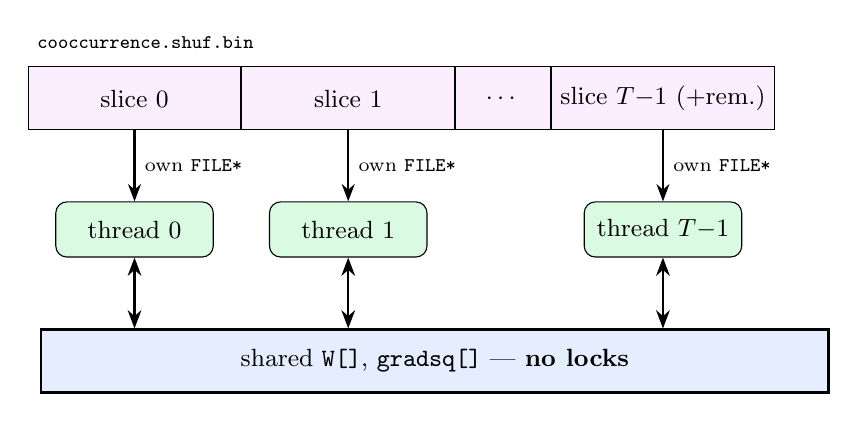
\begin{tikzpicture}[font=\small,
  sl/.style={draw,minimum height=8mm,minimum width=27mm,fill=stageC},
  th/.style={draw,rounded corners,fill=stageD,minimum width=20mm,minimum height=7mm}]
  \node[sl] (s0) at (0,0) {slice 0};
  \node[sl,right=0 of s0] (s1) {slice 1};
  \node[sl,right=0 of s1,minimum width=12mm] (sd) {$\cdots$};
  \node[sl,right=0 of sd] (s3) {slice $T{-}1$ (+rem.)};
  \node[above=1mm of s0.north west,anchor=south west,font=\ttfamily\scriptsize] {cooccurrence.shuf.bin};
  \node[th,below=9mm of s0] (t0) {thread 0};
  \node[th,below=9mm of s1] (t1) {thread 1};
  \node[th,below=9mm of s3] (t3) {thread $T{-}1$};
  \foreach \a/\b in {s0/t0,s1/t1,s3/t3} \draw[arr] (\a) -- node[right,font=\scriptsize]{own \texttt{FILE*}} (\b);
  \node[draw,thick,fill=wA!15,minimum width=100mm,minimum height=8mm,below=9mm of t1.south,xshift=11mm] (W) {shared \texttt{W[]}, \texttt{gradsq[]} --- \textbf{no locks}};
  \foreach \t in {t0,t1,t3} \draw[{Stealth}-{Stealth},thick] (\t) -- (\t |- W.north);
\end{tikzpicture}

\vspace{2mm}
\small
\begin{columns}[T]
\column{0.5\textwidth}
\begin{itemize}
  \item Each epoch: spawn $T$ POSIX threads (pthreads), \texttt{fseeko} each one to its slice, then join.
  \item Each update touches only $2(d{+}1)$ of the $2V(d{+}1)$ entries.
\end{itemize}
\column{0.5\textwidth}
\begin{itemize}
  \item Collisions are rare and only cost a stale or lost update, which SGD tolerates.
  \item \alert{Multithreaded runs are not bit-reproducible}, even with \opt{seed}.
\end{itemize}
\end{columns}
\end{frame}

\begin{frame}{What gets written}
\begin{columns}[c]
\column{0.55\textwidth}
\centering
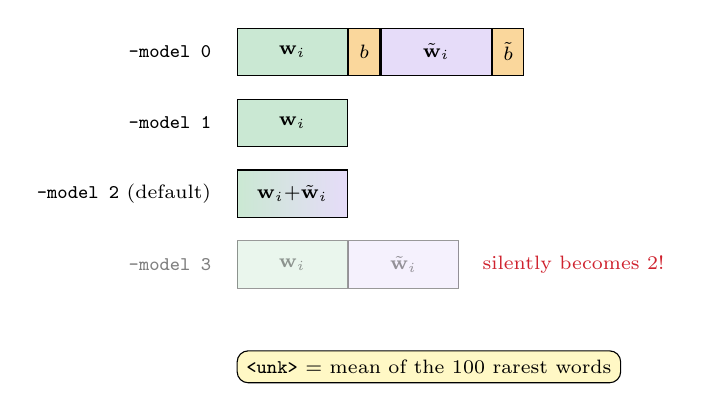
\begin{tikzpicture}[font=\scriptsize,
  v/.style={draw,minimum height=6mm,minimum width=14mm,fill=wC!25},
  c/.style={draw,minimum height=6mm,minimum width=14mm,fill=wE!20},
  b/.style={draw,minimum height=6mm,minimum width=4mm,fill=wB!45}]
  \node[anchor=east] at (-0.2,0) {\texttt{-model 0}};
  \node[v,anchor=west] (a) at (0,0) {$\wv_i$}; \node[b,anchor=west] (ab) at (a.east) {$b$};
  \node[c,anchor=west] (ac) at (ab.east) {$\cv_i$}; \node[b,anchor=west] at (ac.east) {$\tilde b$};
  \node[anchor=east] at (-0.2,-0.9) {\texttt{-model 1}};
  \node[v,anchor=west] at (0,-0.9) {$\wv_i$};
  \node[anchor=east] at (-0.2,-1.8) {\texttt{-model 2} (default)};
  \node[draw,minimum height=6mm,minimum width=14mm,left color=wC!25,right color=wE!20,anchor=west] at (0,-1.8) {$\wv_i{+}\cv_i$};
  \node[anchor=east,gray] at (-0.2,-2.7) {\texttt{-model 3}};
  \node[v,anchor=west,opacity=0.4] (m3) at (0,-2.7) {$\wv_i$}; \node[c,anchor=west,opacity=0.4] at (m3.east) {$\cv_i$};
  \node[warn,anchor=west] at (3.0,-2.7) {silently becomes 2!};
  % unk
  \node[draw,rounded corners,fill=stageB,align=center,anchor=west] at (0,-4) {\texttt{<unk>} = mean of the 100 rarest words};
\end{tikzpicture}
\column{0.45\textwidth}\small
\begin{itemize}
  \item \opt{binary}: 0 = text, 1 = raw \texttt{W} dump ($2V\times(d{+}1)$ doubles), 2 = both.
  \item \opt{write-header} 1 writes ``$V$ $d$'' for gensim (the count excludes \texttt{<unk>}).
  \item The \texttt{<unk>} row is a proxy for unseen words, which is why \texttt{<unk>} is banned from the corpus.
\end{itemize}
\end{columns}
\end{frame}

\begin{frame}{Checkpoints and exact resume}
\centering
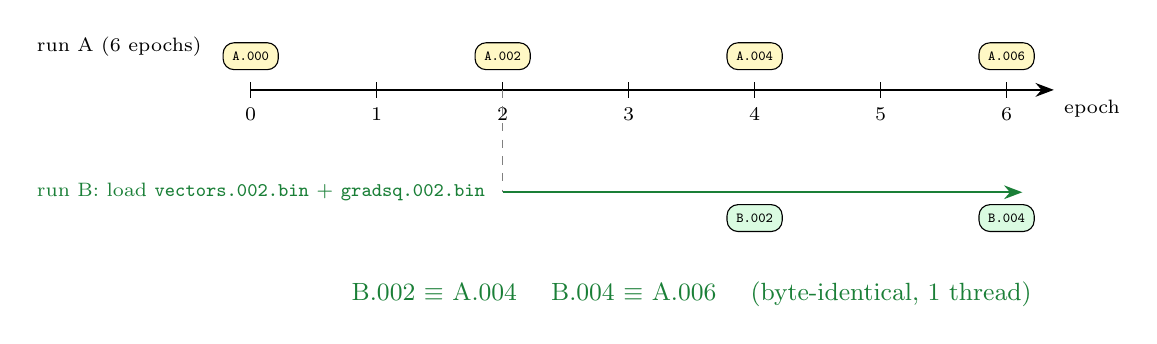
\begin{tikzpicture}[font=\scriptsize]
  \draw[thick,-{Stealth}] (0,0) -- (10.2,0) node[below right]{epoch};
  \foreach \e in {0,...,6} {\draw (\e*1.6,0.1) -- (\e*1.6,-0.1); \node[below] at (\e*1.6,-0.1) {\e};}
  \foreach \e in {0,2,4,6} \node[draw,fill=stageB,rounded corners,above,font=\tiny\ttfamily] at (\e*1.6,0.25) {A.00\e};
  \node[anchor=east,font=\scriptsize] at (-0.5,0.55) {run A (6 epochs)};
  % run B
  \draw[thick,okc,-{Stealth}] (3.2,-1.3) -- (9.8,-1.3);
  \node[okc,left] at (3.1,-1.3) {run B: load \texttt{vectors.002.bin} + \texttt{gradsq.002.bin}};
  \foreach \e/\l in {4/002,6/004} \node[draw,fill=stageD,rounded corners,below,font=\tiny\ttfamily] at (\e*1.6,-1.45) {B.\l};
  \draw[dashed,gray] (3.2,0) -- (3.2,-1.3);
  \node[okc,font=\small] at (5.6,-2.6) {B.002 $\equiv$ A.004 \quad B.004 $\equiv$ A.006 \quad (byte-identical, 1 thread)};
\end{tikzpicture}

\vspace{4mm}
\small
\begin{itemize}
  \item \opt{checkpoint-every} $k$, \opt{save-init-param} (writes epoch 000), \opt{gradsq-file}.
  \item Resume with \opt{load-init-param} 1 and \opt{load-init-gradsq} 1. This is verified by \file{randomization.test.sh}.
\end{itemize}
\end{frame}

% =====================================================================
\section{Operating GloVe}
% =====================================================================

\begin{frame}{The knobs that matter}
\scriptsize
\begin{tabular}{@{}llrp{58mm}@{}}
\toprule
tool & flag & default & guidance\\
\midrule
vocab\_count & \opt{min-count} & 1 & 5 for text8; 20 for Wiki+Gigaword\\
             & \opt{max-vocab} & none & 1.2M for the Dolma run\\
\midrule
cooccur & \opt{window-size} & 15 & small: syntax; large: topic (10 in 2024 runs)\\
        & \opt{symmetric}, \opt{distance-weighting} & 1, 1 & left-only / unweighted variants\\
        & \opt{memory} & 3 GB & help says 4; affects speed, not the result\\
\midrule
shuffle & \opt{memory}, \opt{seed} & 2 GB, time & set \opt{seed} for reproducibility\\
\midrule
glove & \opt{vector-size} & 50 & 50--300\\
      & \opt{iter} & 25 & 50--100 for large corpora\\
      & \opt{eta} & 0.05 & applies to vectors only, not biases\\
      & \opt{x-max}, \opt{alpha} & 100, 0.75 & $x_{\max}\approx 10$ for small corpora\\
      & \opt{threads} & 8 & use 1 for bit-reproducibility\\
\bottomrule
\end{tabular}
\end{frame}

\begin{frame}{Sizing a run}
\begin{columns}[c]
\column{0.5\textwidth}
\centering
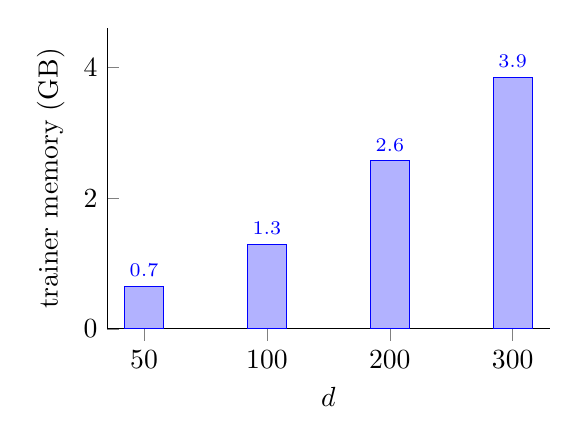
\begin{tikzpicture}
\begin{axis}[width=7.2cm,height=5.4cm,ybar,bar width=14pt,
  symbolic x coords={50,100,200,300},xtick=data,xlabel={$d$},
  ylabel={trainer memory (GB)},ymin=0,ymax=4.6,
  nodes near coords,nodes near coords style={font=\scriptsize,/pgf/number format/.cd,fixed,precision=1},
  axis lines*=left,every axis plot/.append style={fill=accent!60,draw=accent}]
  \addplot coordinates {(50,0.65) (100,1.29) (200,2.57) (300,3.85)};
\end{axis}
\end{tikzpicture}

{\scriptsize $V=400$k: $\;2\cdot 2V(d{+}1)\cdot 8$ bytes (\texttt{W} + \texttt{gradsq})}
\column{0.5\textwidth}\small
\begin{itemize}
  \item \textbf{Disk}: $16\cdot\mathrm{nnz}(X)$ for each co-occurrence file. While shuffling there are input, temp, and output copies, so plan for about $3\times$.
  \item \textbf{Time per epoch}: $O(\mathrm{nnz}(X)\cdot d)$. The paper finds that nnz grows sub-linearly in corpus size (about $|C|^{0.8}$).
  \item \textbf{I/O (input/output)}: every stage streams sequentially. \texttt{glove} re-reads the whole file every epoch, so a solid-state drive (SSD) or the page cache helps.
\end{itemize}
\end{columns}
\end{frame}

\begin{frame}{Evaluation: word analogies}
\begin{columns}[c]
\column{0.5\textwidth}
\centering
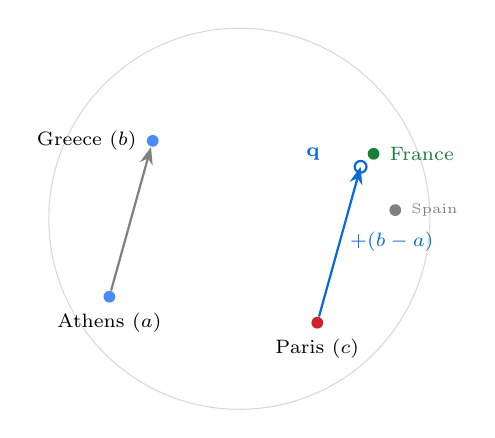
\begin{tikzpicture}[scale=1.1,pt/.style={circle,fill,inner sep=1.5pt}]
  \draw[gray!30] (0,0) circle (2.2);
  \node[pt,wA,label={[font=\scriptsize]below:Athens ($a$)}] (a) at (-1.5,-0.9) {};
  \node[pt,wA,label={[font=\scriptsize]left:Greece ($b$)}] (b) at (-1.0,0.9) {};
  \node[pt,wD,label={[font=\scriptsize]below:Paris ($c$)}] (c) at (0.9,-1.2) {};
  \coordinate (q) at (1.4,0.6);
  \node[pt,okc,label={[font=\scriptsize,okc]right:France}] at (1.55,0.75) {};
  \node[pt,gray,label={[font=\tiny,gray]right:Spain}] at (1.8,0.1) {};
  \draw[arr,gray] (a) -- (b);
  \draw[arr,accent,thick] (c) -- node[right,font=\scriptsize]{$+(b-a)$} (q);
  \node[draw,accent,circle,inner sep=1.5pt,thick] at (q) {};
  \node[font=\scriptsize,accent] at (0.85,0.75) {$\mathbf q$};
\end{tikzpicture}
\column{0.5\textwidth}\small
\begin{enumerate}
  \item L2-normalise every vector.
  \item $\mathbf q=\hat\wv_b-\hat\wv_a+\hat\wv_c$.
  \item Predict $\arg\max_x \hat\wv_x^\top\mathbf q$, \alert{excluding $a,b,c$}.
  \item Report top-1 accuracy, split into semantic (5 files) and syntactic (9 files).
\end{enumerate}
\vspace{2mm}
\file{eval/python/evaluate.py} batches 100 questions per matrix product.
\file{distance.py} and \file{word\_analogy.py} are interactive tools.
\end{columns}
\end{frame}

\begin{frame}{Quirks found while reading the code}
\small
\begin{itemize}
  \item[\textcolor{warn}{\textbullet}] \textbf{\opt{model} 3 is unreachable}: \file{glove.c:523} maps everything except 0 and 1 to 2.
  \item[\textcolor{warn}{\textbullet}] \textbf{Bias updates ignore \opt{eta}} and are not clipped.
  \item[\textcolor{warn}{\textbullet}] \textbf{Defaults vs.\ help}: \texttt{cooccur} defaults to 3 GB and \texttt{shuffle} to 2 GB; both help texts say 4.
  \item[\textcolor{warn}{\textbullet}] \textbf{NaN guard vs.\ gradsq}: a rejected vector update has already incremented \texttt{gradsq}.
  \item[\textcolor{warn}{\textbullet}] \textbf{\texttt{-Ofast}} disables the NaN checks (\texttt{-ffinite-math-only}); the Makefile uses \texttt{-O3}.
  \item[\textcolor{warn}{\textbullet}] \textbf{Help invocation}: \texttt{cooccur}/\texttt{glove} print help with no arguments; \texttt{vocab\_count}/\texttt{shuffle} need \texttt{-h}.
  \item[\textcolor{warn}{\textbullet}] \textbf{Out-of-vocabulary (OOV) tokens are skipped}, so window distances count only in-vocabulary tokens.
\end{itemize}
\end{frame}

% =====================================================================
\section{Summary}
% =====================================================================

\begin{frame}{GloVe in one picture}
\centering
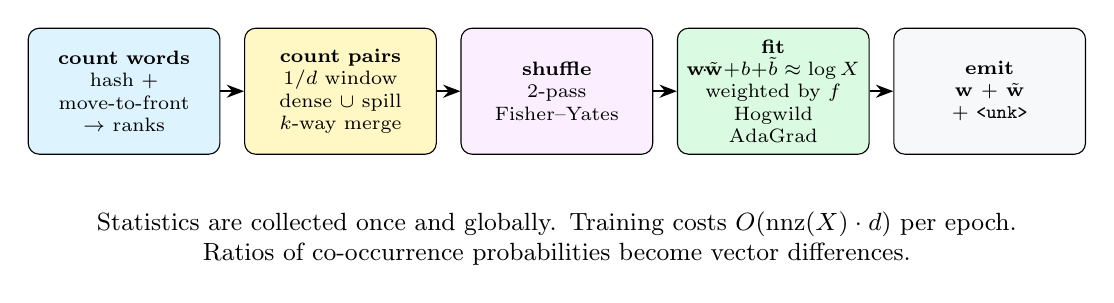
\begin{tikzpicture}[font=\scriptsize,node distance=3mm,
  s/.style={draw,rounded corners,align=center,minimum height=16mm,text width=22mm}]
  \node[s,fill=stageA] (a) {\textbf{count words}\\hash +\\move-to-front\\$\to$ ranks};
  \node[s,fill=stageB,right=of a] (b) {\textbf{count pairs}\\$1/d$ window\\dense $\cup$ spill\\$k$-way merge};
  \node[s,fill=stageC,right=of b] (c) {\textbf{shuffle}\\2-pass\\Fisher--Yates};
  \node[s,fill=stageD,right=of c] (d) {\textbf{fit}\\$\wv\!\cdot\!\cv+b+\tilde b\approx\log X$\\weighted by $f$\\Hogwild AdaGrad};
  \node[s,fill=fileC,right=of d] (e) {\textbf{emit}\\$\wv+\cv$\\+ \texttt{<unk>}};
  \foreach \x/\y in {a/b,b/c,c/d,d/e} \draw[arr] (\x) -- (\y);
  \node[below=6mm of c,text width=120mm,align=center,font=\small]
   {Statistics are collected \alert{once} and globally. Training costs $O(\mathrm{nnz}(X)\cdot d)$ per epoch.\\
    Ratios of co-occurrence probabilities become \alert{vector differences}.};
\end{tikzpicture}
\end{frame}

\begin{frame}{References}
\small
\begin{enumerate}
  \item J.~Pennington, R.~Socher, C.~D.~Manning. \emph{GloVe: Global Vectors for Word Representation}. Empirical Methods in Natural Language Processing (EMNLP) 2014.
  \item T.~Mikolov et al. \emph{Distributed Representations of Words and Phrases and their Compositionality}. Neural Information Processing Systems (NeurIPS) 2013.
  \item J.~Duchi, E.~Hazan, Y.~Singer. \emph{Adaptive Subgradient Methods} (AdaGrad). Journal of Machine Learning Research (JMLR) 2011.
  \item B.~Recht, C.~R\'e, S.~Wright, F.~Niu. \emph{Hogwild!} NeurIPS 2011.
  \item \url{https://nlp.stanford.edu/projects/glove/} --- pre-trained vectors and the paper.
  \item Companion document: \file{docs/architecture/glove\_architecture.pdf}.
\end{enumerate}
\end{frame}

\end{document}
